\documentclass[uplatex, twocolumn,10pt]{jsarticle}

\usepackage[dvipdfmx]{graphicx}
\usepackage{latexsym}
\usepackage{bmpsize}
\usepackage{url}
\usepackage{comment}

\def\Underline{\setbox0\hbox\bgroup\let\\\endUnderline}
\def\endUnderline{\vphantom{y}\egroup\smash{\underline{\box0}}\\}

\newcommand{\ttt}[1]{\texttt{#1}}

\begin{document}

\title{\bf{\LARGE{Sample of \LaTeX  Document} \\ \Large{\LaTeX のサンプルコード}}}
\author{平木場 風太\\宮崎大学大学院}
\date{2019年6月12日(水)}

\maketitle

\section{はじめに}
\begin{figure}[t]
  \begin{center}
    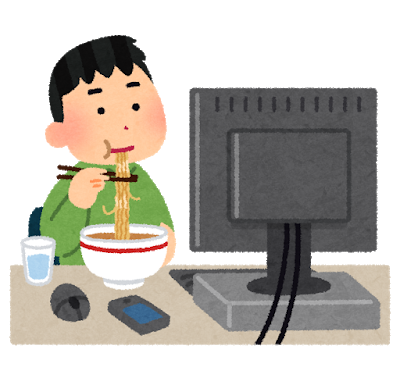
\includegraphics[width=7cm]{img/syokuji_computer.png}
    \caption{パソコンの前でご飯を食べる人のイラスト}
    \label{fig:syokuji_computer}
  \end{center}
\end{figure}

パソコンの前でご飯を食べることはよくある。パソコンの前でご飯を食べる人のイラストを図\ref{fig:syokuji_computer}に示す。
このイラストは、規約の範囲内であれば、個人、法人、商用、非商用問わず無料で利用できることでおなじみの、{\bf かわいいフリー素材 いらすとや}\cite{irasutoya}より引用した。

\section{おわりに}
やっぱり{\bf いらすとや}のイラストはすばらしい。

\begin{thebibliography}{99}
  \bibitem{irasutoya} いらすとや, last access 2019.6.13 \url{https://www.irasutoya.com/}

\end{thebibliography}

\end{document}
